\documentclass[a4paper,11pt]{article}

% \usepackage[smartEllipses]{markdown}
% \usepackage[hashEnumerators,smartEllipses]{markdown}
% \usepackage[hashEnumerators,smartEllipses,hybrid]{markdown}
\usepackage[hybrid]{markdown}
\usepackage[export]{adjustbox} % рамки вокруг фото
\usepackage{minted} % Для вставки кода
% \usepackage{xpatch}
% \xpretocmd{\inputminted}{\par\vspace{1em}}{}{}
% \xapptocmd{\inputminted}{\par\vspace{1em}}{}{}
% \usepackage{indentfirst}
% \setlength{\parindent}{0pt} % Отключает отступ в начале каждого абзаца
\usepackage{parskip} % убрать красную строку и добавить вертикальный отступ между абзацами


%%% Мои команды
\newcommand{\insertMyCode}[2]{ % вставка кода
    % #1 — язык
    % #2 — путь до файла
    \inputminted[
    % framesep=2mm,
    baselinestretch=1.2,
    bgcolor=LightGray!30,
    fontsize=\footnotesize,
    linenos
    ]{#1}{#2}
}


%%% Работа с русским языком
\usepackage{cmap} % поиск в PDF
\usepackage{mathtext} % русские буквы в фомулах
\usepackage[T2A]{fontenc} % кодировка
\usepackage[utf8]{inputenc} % кодировка исходного текста
\usepackage[english,russian]{babel} % локализация и переносы

%%% Дополнительная работа с математикой
\usepackage{amsmath,amsfonts,amssymb,amsthm,mathtools} % AMS
\usepackage{icomma} % "Умная" запятая: $0,2$ —- число, $0, 2$ —- перечисление

%%% Перенос знаков в формулах (по Львовскому)
\newcommand*{\hm}[1]{#1\nobreak\discretionary{}
{\hbox{$\mathsurround=0pt #1$}}{}}

%%% Работа с картинками
\usepackage{graphicx} % Для вставки рисунков
\graphicspath{{images/}} % папки с картинками
% \setlength\fboxsep{3pt} % Отступ рамки \fbox{} от рисунка
% \setlength\fboxrule{1pt} % Толщина линий рамки \fbox{}
% \usepackage{wrapfig} % Обтекание рисунков текстом

%%% Работа с таблицами
\usepackage{array,tabularx,tabulary,booktabs} % Дополнительная работа с таблицами
\usepackage{longtable} % Длинные таблицы
\usepackage{multirow} % Слияние строк в таблице

%%% Теоремы
% \theoremstyle{plain} % Это стиль по умолчанию, его можно не переопределять.
\newtheorem{theorem}{Теорема}[section]
\newtheorem{proposition}[theorem]{Утверждение}

\theoremstyle{definition} % "Определение"
\newtheorem{corollary}{Следствие}[theorem]
\newtheorem{problem}{Задача}[section]

\theoremstyle{remark} % "Примечание"
\newtheorem*{nonum}{Решение}

%%% Программирование
\usepackage{etoolbox} % логические операторы

%%% Страница
% \usepackage{extsizes} % Возможность сделать 14-й шрифт % конфликт с parskip
\usepackage{geometry} % Простой способ задавать поля
\geometry{top=25mm}
\geometry{bottom=35mm}
\geometry{left=20mm}
\geometry{right=20mm}

\usepackage{fancyhdr} % Колонтитулы
\pagestyle{fancy}
\renewcommand{\headrulewidth}{0mm} % Толщина линейки, отчеркивающей верхний колонтитул
% \lfoot{Нижний левый}
% \rfoot{Нижний правый}
% \rhead{Верхний правый}
% \chead{Верхний в центре}
% \lhead{Верхний левый}
\cfoot % По умолчанию здесь номер страницы

\usepackage{lastpage} % Узнать, сколько всего страниц в документе.

\usepackage{soul} % Модификаторы начертания

\usepackage{setspace} % Интерлиньяж
%\onehalfspacing % Интерлиньяж 1.5
%\doublespacing % Интерлиньяж 2
%\singlespacing % Интерлиньяж 1

\usepackage{hyperref}
\usepackage[usenames,dvipsnames,svgnames,table,rgb]{xcolor}
\hypersetup{ % Гиперссылки
unicode=true, % русские буквы в раздела PDF
pdftitle={Заголовок}, % Заголовок
pdfauthor={Автор}, % Автор
pdfsubject={Тема}, % Тема
pdfcreator={Создатель}, % Создатель
pdfproducer={Производитель}, % Производитель
pdfkeywords={keyword1} {key2} {key3}, % Ключевые слова
colorlinks=true, % false: ссылки в рамках; true: цветные ссылки
linkcolor=red, % внутренние ссылки
citecolor=green, % на библиографию
filecolor=magenta, % на файлы
urlcolor=cyan % на URL
}

\usepackage{multicol} % Несколько колонок

%%% Хз что это (потом разобраться)
% \usepackage{upgreek}
\usepackage{cite}
\usepackage{csquotes} % Еще инструменты для ссылок
%Смотри источник 1 \cite{qwerty,Fama,Fama2}.
%\renewcommand{\refname}{Список источников}  % По умолчанию %"Список литературы" (article)
%\renewcommand{\bibname}{Литература}  % По умолчанию "Литература" (book и report)
%\renewcommand{\familydefault}{\sfdefault} % Начертание шрифта

\begin{document}


\begin{titlepage} % начало титульной страницы
\pagestyle{empty}
\begin{center}

\Large
\textbf{Федеральное государственное автономное образовательное учреждение высшего образования\\
«Национальный исследовательский университет\\
«Высшая школа экономики»}\\
\vspace{5mm}

\Large
Образовательная программа \\
«Прикладная математика»
\vspace{40mm}

\Large
\textbf{ОТЧЕТ} \\
\textbf{По лабораторной работе № 1} \\
\vspace{5mm}
\Large По предмету \\
\LARGE\textbf{«Численные методы»} \\
\vspace{5mm}
\Large По теме \\
\LARGE\textbf{«Теория погрешностей и машинная арифметика»}
\end{center}

\begin{center}
\vfill

\large
\begin{flushright}
\textbf{Выполнил} \\
студент группы БПМ211 \\
Кудряшов Максим Дмитриевич \\
\end{flushright}

\large
\begin{flushright}
\textbf{Проверил} \\
Брандышев Петр Евгеньевич \\
\end{flushright}

\large
\vspace{20mm}
Москва - 2024
\end{center}
\end{titlepage} % конец титульной страницы

\newpage
\tableofcontents
\newpage

\section{Расчет погрешности частичных сумм ряда (№ 1.1.8)}

\subsection{Формулировка задания}

1. Найти сумму ряда $S$ аналитически.

$$S = \sum\limits_{n=0}^\infty \frac{32}{n^2+9n+20}$$

2. Найти частичные суммы ряда $S_N$ при $N = 10, 10^2, 10^3, 10^4, 10^5$.

$$S_N = \sum\limits_{n=0}^N \frac{32}{n^2+9n+20}$$

3. Вычислить погрешности для каждого N.

4. Вычислить количество значащих цифр для каждого N.

5. Построить гистограмму зависимости верных цифр результата от $N$.

\subsection{Найдем сумму ряда аналитически}

Посчитаем значение предела в Wolfram:

\begin{figure}[h]
\frame{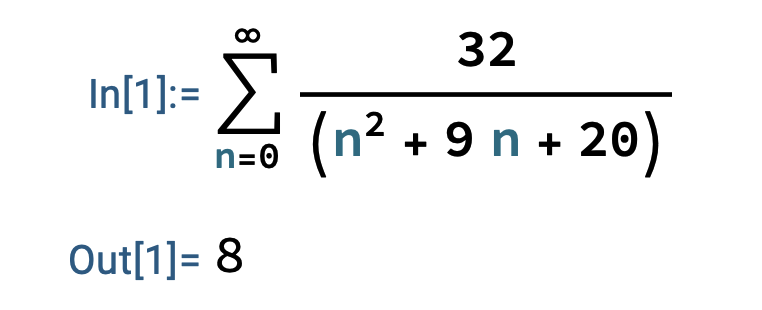
\includegraphics[width=0.3\linewidth]{../../calculate_sum/wolfram}}
\end{figure}

Итого $S = \sum\limits_{n=0}^\infty \frac{32}{n^2+9n+20} = 8$

\subsection{Найдем погрешности}

Для различных значений N вычислим частичные суммы, погрешности и количество значащих цифр.

\subsubsection{Код на Python}

\insertMyCode{python3}{../calculate_sum/calculate_sum.py}

\subsubsection{Посчитанные данные}

\begin{tabular}{lrrrr}
\toprule
 & N & Значение & Погрешность & Число значащих цифр \\
\midrule
0 & 10 & 5.714286 & 2.285714 & 0 \\
1 & 100 & 7.692308 & 0.307692 & 1 \\
2 & 1000 & 7.968127 & 0.031873 & 2 \\
3 & 10000 & 7.996801 & 0.003199 & 3 \\
4 & 100000 & 7.999680 & 0.000320 & 4 \\
\bottomrule
\end{tabular}


\subsubsection{Визуализация посчитанных данных}

\begin{figure}[h]
    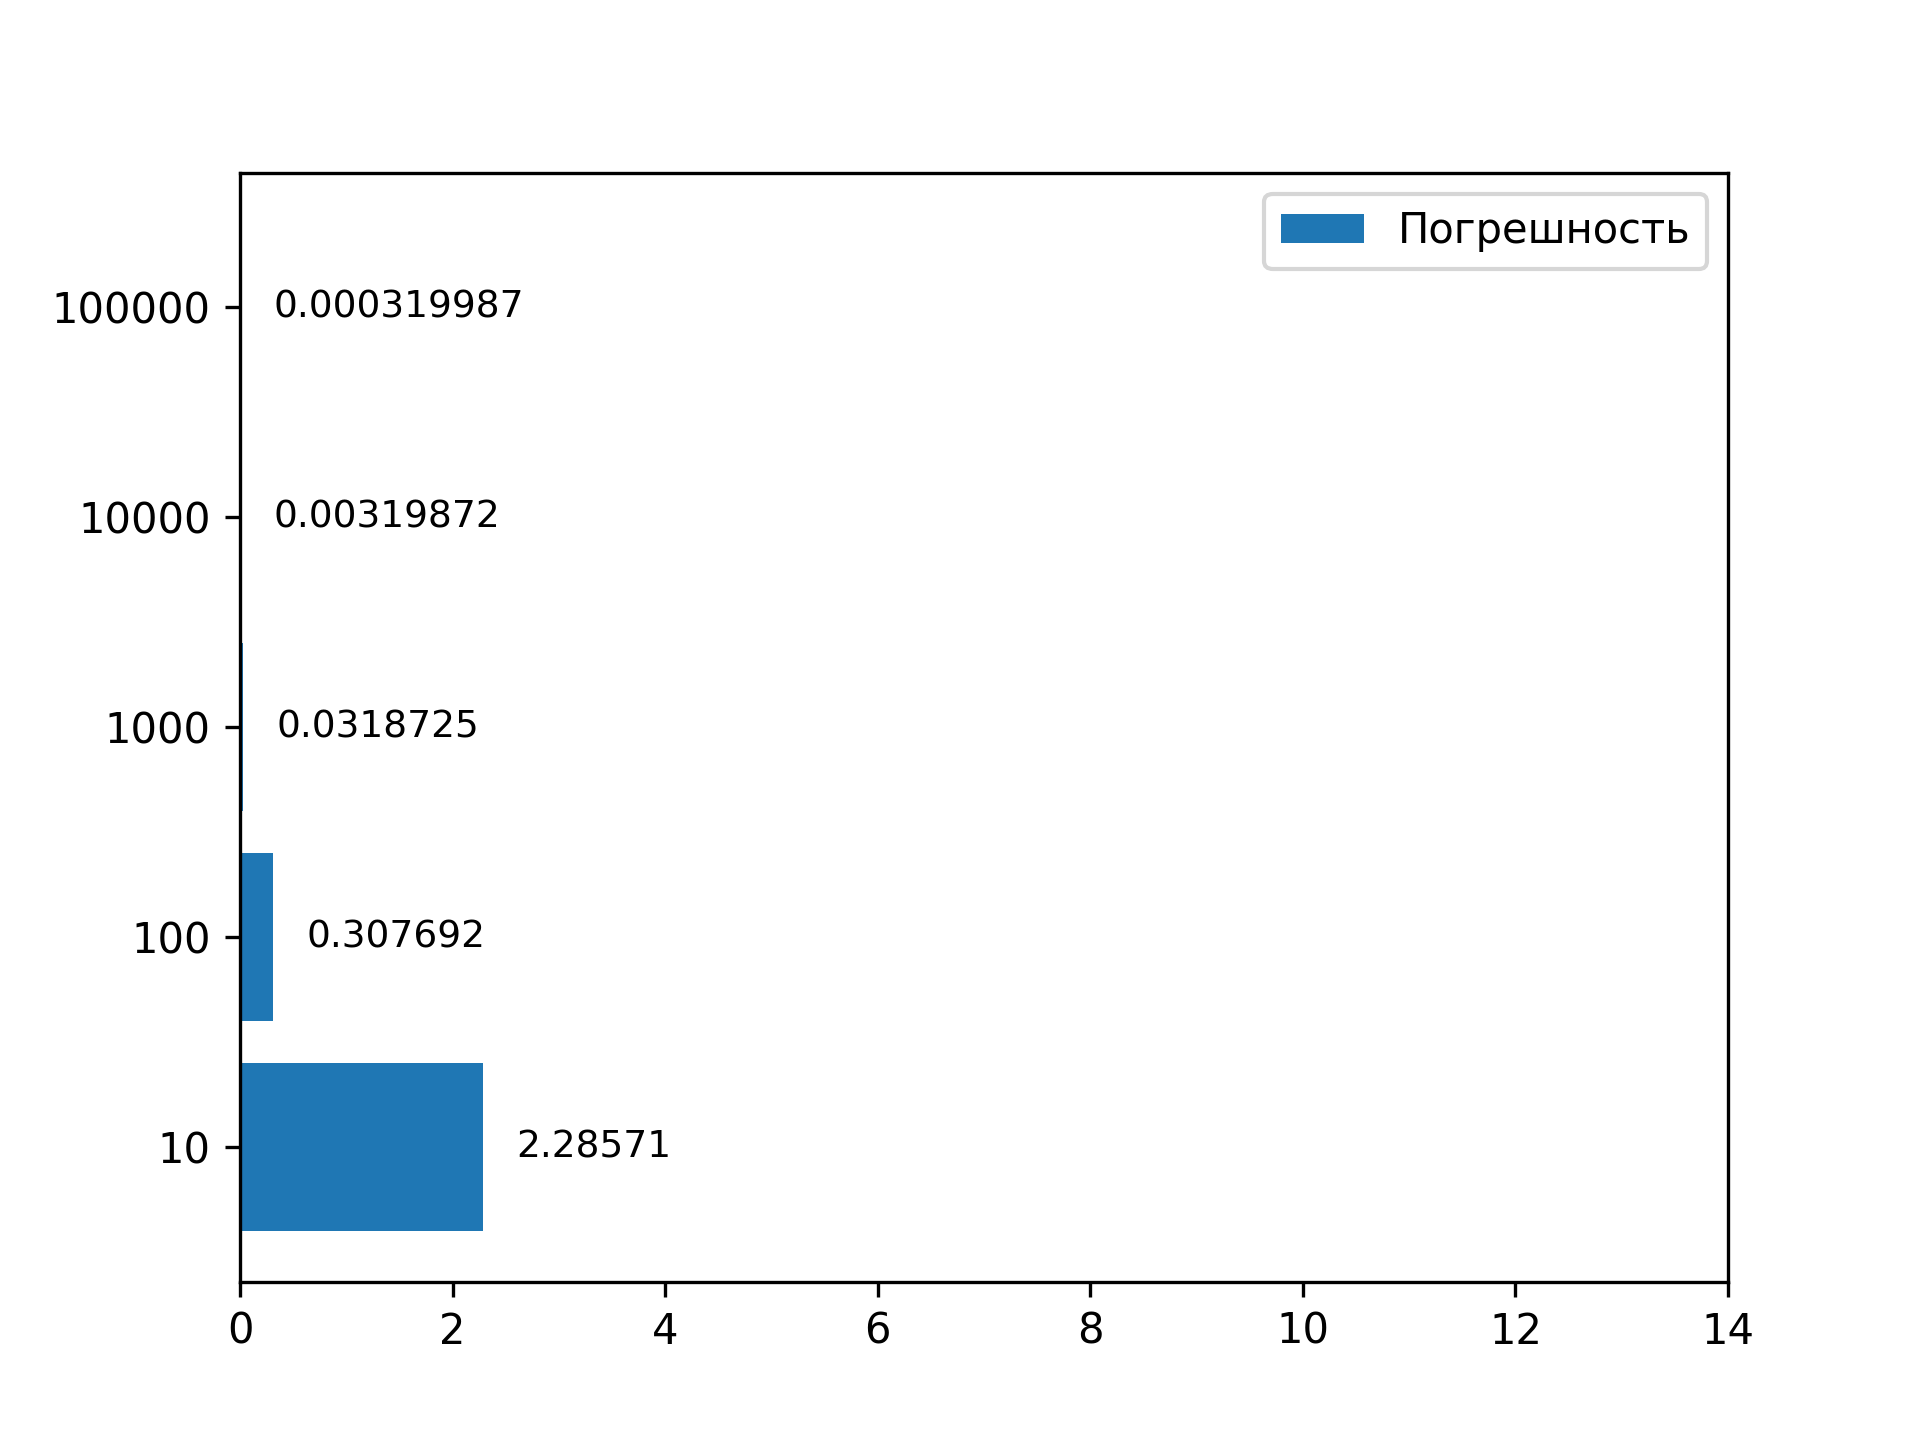
\includegraphics[width=0.49\linewidth]{../../calculate_sum/errors}
    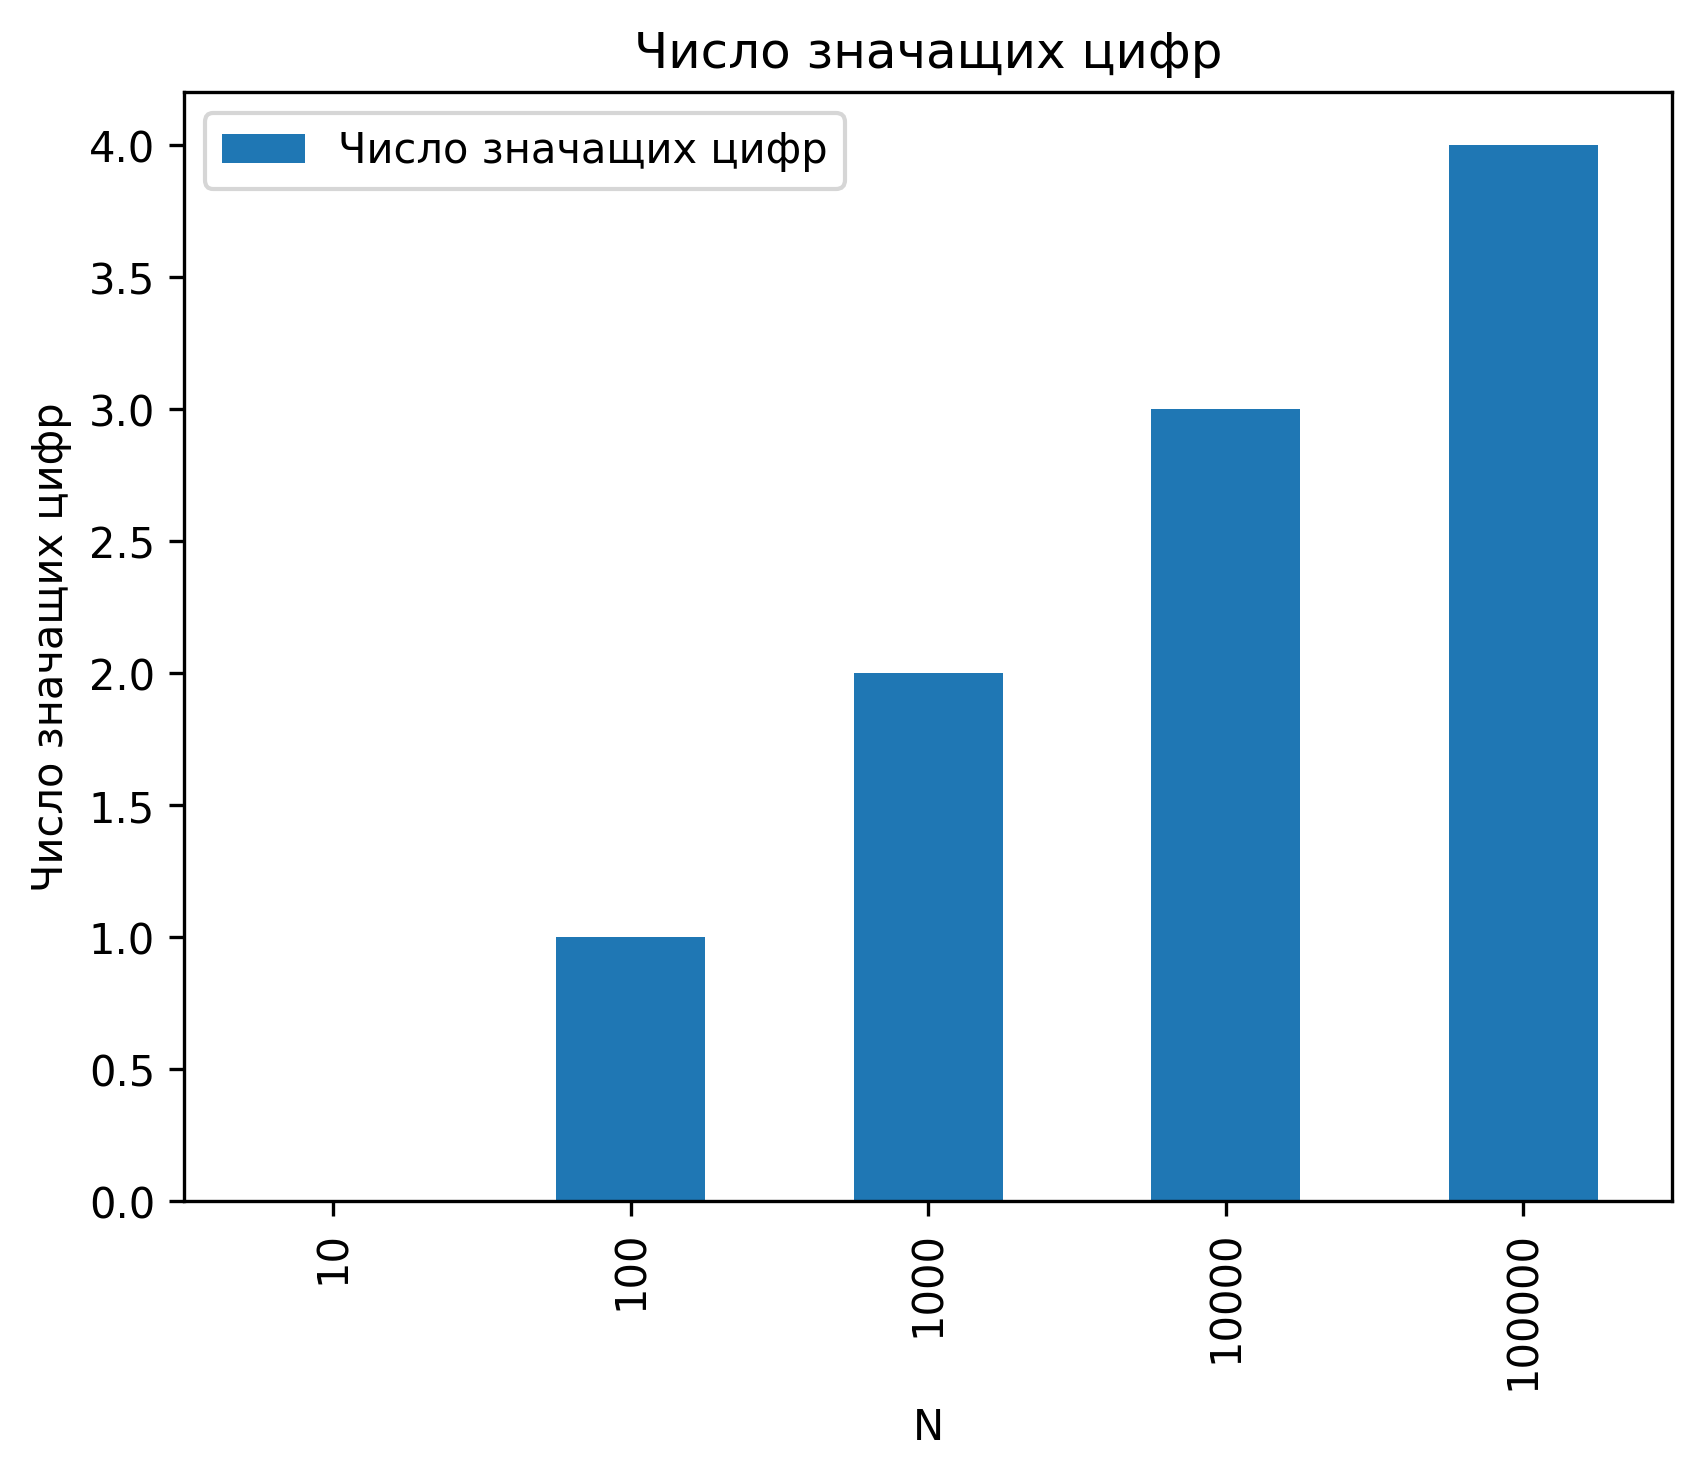
\includegraphics[width=0.49\linewidth]{../../calculate_sum/digits}
\end{figure}

\newpage
\section{Квадратное уравнение (№ 1.5.2)}
\subsection{Формулировка задания}

Дано квадратное уравнение. Предполагается, что один из коэффициентов уравнения (в индивидуальном варианте помечен *) получен в результате округления. Произвести теоретическую оценку погрешностей корней в зависимости от погрешности коэффициента. Вычислить корни уравнения при нескольких различных значениях коэффициента в пределах заданной точности. Сравнить полученные результаты.

$$a x^2+bx+c^* = 0$$
$$a = 1$$
$$b = 27.4$$
$$c^* = 187.65 $$

\subsection{Нахождение погрешности}

В общем случае:

$$x^* = x \pm \Delta x$$
$$\bar{\Delta} x = |x| \bar{\delta} x$$
$$\bar{\Delta} f(x) = |f'(x)| \bar{\Delta} x$$
$$ \bar{\delta} f(x) = \frac{\bar{\Delta} f(x)}{|f(x)|} = \frac{|f'(x)| \bar{\Delta} x}{|f(x)|} = \frac{|f'(x)| |x| \bar{\delta} x}{|f(x)|}$$

Итого:

$$ \bar{\delta} f(x) = \frac{|f'(x)| |x|}{|f(x)|} \bar{\delta} x$$

В других обобзначениях:

$$ \bar{\delta} x(c) = \frac{|x'(c)| |c|}{|x(c)|} \bar{\delta} c$$

Найдем производную и значение функции:

$$x = \frac{-b \pm \sqrt{b^2-4ac}}{2a} $$

$$x_1 = -13.9, x_2 = -13.5$$

$$x'(c) = -\frac{1}{\sqrt{b^2-4ac}} = -2.5$$

Подставим:

$$ \bar{\delta} x_1 = \frac{2.5 \cdot 187.65}{13.9} \cdot \bar{\delta} c = 33.75 \cdot \bar{\delta} c$$

$$ \bar{\delta} x_2 = \frac{2.5 \cdot 187.65}{13.5} \cdot \bar{\delta} c = 34.75 \cdot \bar{\delta} c$$

Найдем погрешности корней при разных погрешностях $c$:

\subsection{Код на Python}

\insertMyCode{python3}{../quadratic_equation/quadratic_equation.py}

\subsection{Результат работы программы}

\begin{minted}{text}
x1 = (-13.7+0.24494897427828197j), x2 = (-13.7-0.24494897427828197j), error = 0.1
x1 = -13.87320508075684,	x2 = -13.526794919243159,	error = 0.01
x1 = -13.897484176581239,	x2 = -13.50251582341876,	error = 0.001
x1 = -13.899749843554309,	x2 = -13.500250156445688,	error = 0.0001
x1 = -13.899974998437234,	x2 = -13.500025001562767,	error = 1e-05
x1 = -13.899997499984318,	x2 = -13.50000250001568,	error = 1e-06
x1 = -13.899999749999795,	x2 = -13.500000250000204,	error = 1e-07
x1 = -13.899999974999915,	x2 = -13.500000025000084,	error = 1e-08
x1 = -13.899999997499963,	x2 = -13.500000002500036,	error = 1e-09
x1 = -13.899999999749967,	x2 = -13.500000000250031,	error = 1e-10
x1 = -13.899999999974925,	x2 = -13.500000000025073,	error = 1e-11
x1 = -13.89999999999745,	x2 = -13.500000000002547,	error = 1e-12
x1 = -13.899999999999652,	x2 = -13.500000000000346,	error = 1e-13
x1 = -13.899999999999936,	x2 = -13.500000000000062,	error = 1e-14
x1 = -13.899999999999936,	x2 = -13.500000000000062,	error = 1e-15
x1 = -13.899999999999936,	x2 = -13.500000000000062,	error = 1e-16
x1 = -13.899999999999936,	x2 = -13.500000000000062,	error = 1e-17
x1 = -13.899999999999936,	x2 = -13.500000000000062,	error = 1e-18
x1 = -13.899999999999936,	x2 = -13.500000000000062,	error = 1e-19
x1 = -13.899999999999936,	x2 = -13.500000000000062,	error = 1e-20
\end{minted}


\newpage
\section{Нахождение машиннного нуля (№ 1.6, 1.7)}

\subsection{Формулировка задания}

Вычислить значения машинного нуля, машинной бесконечности, машинного эпсилон в режимах одинарной, двойной и расширенной точности на двух алгоритмических языках. Сравнить результаты.

\subsection{Теория}

Машинная бесконечность $X_\infty = 2^n$ , где n - первое натуральное число, при котором происходит переполнение.

Машинный ноль $X_0 = 2^{-n}$ , где n - первое натуральное число, при котором $2^{-n}$ совпадает с нулем.

Машинная эпсилон $\varepsilon_M = 2^{-n}$ , где n - наибольшее натуральное число, при котором сумма вычисленного значения $1 + 2^{-n}$ еще больше 1.

\subsection{Код на Python}

\insertMyCode{python3}{../machine_values/machine_values.py}

\subsection{Код на C++}

\insertMyCode{c++}{../machine_values/machine_values.cpp}

\subsection{Вывод кода на Python}

\begin{minted}{text}
<class 'numpy.float32'> машинный ноль = 2^-150
<class 'numpy.float32'> машинная бесконечность = 2^128
<class 'numpy.float32'> машинное эпсилон = 2^-24

<class 'numpy.float64'> машинный ноль = 2^-1075
<class 'numpy.float64'> машинная бесконечность = 2^1024
<class 'numpy.float64'> машинное эпсилон = 2^-53

<class 'numpy.longdouble'> машинный ноль = 2^-1075
<class 'numpy.longdouble'> машинная бесконечность = 2^1024
<class 'numpy.longdouble'> машинное эпсилон = 2^-53
\end{minted}

\subsection{Вывод кода на C++}

\begin{minted}{text}
float машинный ноль = 2^-150
float машинная бесконечность = 2^128
float машинное эпсилон = 2^-24

double машинный ноль = 2^-1075
double машинная бесконечность = 2^1024
double машинное эпсилон = 2^-53

long double машинный ноль = 2^-1075
long double машинная бесконечность = 2^1024
long double машинное эпсилон = 2^-53
\end{minted}

\subsection{Сравнение результатов}

Видно, что и машинный ноль, и машинное эпсилон, и машинная бесконечность совпадают для Python и для C++.

\newpage
\section{Расчет погрешности матрицы (№ 1.9.2)}

\subsection{Формулировка задания}

Для матрицы $A$ решить вопрос о существовании обратной матрицы в следующих случаях:

1. элементы матрицы заданы точно;

2. элементы матрицы заданы приближенно с относительной погрешностью $\alpha = 0.05$ и $\beta = 0.1$

$$
A =
\begin{pmatrix}
    30 & 34 & 19 \\
    31.4 & 35.4 & 20 \\
    24 & 28 & 13 \\
\end{pmatrix}
$$

\subsection{Теория}

Пусть элементы матрицы определителя заданы приближенно с относительной погрешностью $\delta$. 
Пусть элементы матрицы обозначены через $a_{ij}$.
Тогда каждый элемент матрицы теперь уже не равен конкретному значению, а может принимать любое значение из oтрезка
$[a_{ij} (1 - \delta), a_{ij} (1 + \delta )]$ если $a_{ij} > 0$,
и из отрезка $[a_{ij} (1 + \delta), a_{ij} (1 - \delta )]$ если $a_{ij} < 0$.

Множество всех возможных значений элементов матрицы представляет собой замкнутое ограниченное множество в 9-мерном пространстве. 
Сам определитель является непрерывной и дифференцируемой функцией 9 переменных -- элементов матрицы $a_{ij}$.
По теореме Вейерштрасса эта функция достигает на указанном множестве своего наибольшего и наименьшего значений $M$ и $m$.

Если отрезок $[m, M]$ не содержит точку 0, то это означает, что при всевозможных допустимых значениях элементов матрицы $a_{ij}$
определитель не обращается в 0. 
Если же точка 0 принадлежит отрезку $[m, M]$, такое утверждение будет неправомерным. Будет иметь место неопределённость.

Нахождению значений m и M помогают следующие рассуждения. Как функция своих аргументов (элементов матрицы $a_{ij}$) определитель обладает таким свойством (принцип максимума): 
эта функция достигает своего наибольшего и наименьшего значений всегда на границе области.
Более того, можно доказать, что эти значения достигаются в точках, координаты которых имеют вид $a_{ij} (1 \pm \delta)$.
Таких точек $2ˆ9 = 512$.
В каждой из них следует вычислить определитель, а затем выбрать из полученных значений самое большое и самое маленькое. Это и будут числа $M$ и $m$.

\subsection{Код на Python}

\insertMyCode{python3}{../matrix_det/matrix_det.py}

\subsection{Вывод программы}

Определитель без погрешности 9.600000000000069

Минимальное значение определителя = -984.8728000000016 \\
Максимальное значение определителя = 1027.8990000000008 \\
При относительной погрешности 0.05 определитель может обратиться в 0 

Минимальное значение определителя = -2965.2384 \\
Максимальное значение определителя = 3032.2959999999985 \\
При относительной погрешности 0.1 определитель может обратиться в 0

\subsection{Выводы}

Если значения заданы точно, то определитель не равен 0, а следовательно существует обратная матрица.

Если лементы матрицы заданы приближенно с относительной погрешностью $\alpha = 0.05$ и $\beta = 0.1$, то определитель можно равняться нулю, значит обратная матрица можно не существовать.



\end{document}
